%%%%%%%%%%%%%%%%%%%%%%%%%%%%%%%%%%%%%%%%%%%%%%%%%%%%%%%%%%%%%%%%%%%%%%%%
\chapter{Datasets}\label{chap:datasets}
%%%%%%%%%%%%%%%%%%%%%%%%%%%%%%%%%%%%%%%%%%%%%%%%%%%%%%%%%%%%%%%%%%%%%%%%


\noindent The importance of databases can be demonstrated by looking at the challenges in the field of Artificial Intelligence.
For years, the research on Artificial Intelligence has focused on the same concept: a better algorithm would make better decisions, regardless of the data.
However, even the best algorithm would not work well if the learned data didn't reflect the real world.\\
A good dataset is one that fits the desired purpose.
However, there are some general considerations that indicate good quality in a dataset.
Completeness, balanced classes, good organization, and quality labeling define a dataset of high quality.

In skin detection, a dataset usually consists of two types of pictures: the original images and the labeled images.
Labeled images are the ground truths and can either be binary masks or segmentation masks, where only the skin pixels are present.
Some datasets focus on the skin of a specific body part, such as the face or the abdomen.


%%%%%%%%%%%%%%%%%%%%%%%%%%%%%%%%%%%%%%%%%%%%%%%%%%%%%%%%%%%%%%%%%%%%%%%%
\section{Datasets Overview}
%%%%%%%%%%%%%%%%%%%%%%%%%%%%%%%%%%%%%%%%%%%%%%%%%%%%%%%%%%%%%%%%%%%%%%%%

A summary of common skin detection datasets is presented in \autoref{tab:dataset_table}, starting from the oldest to the newest. Only public datasets featuring images and including ground truths are considered.\\ 
\textbf{TDSD}~\cite{zhu2004adaptive} is the acronym of Test Database for Skin Detection, which is a database featuring 555 full-body skin images. Its ground truths are segmentation masks. It is also referred to as IBTD.\\
\textbf{ECU}~\cite{phung2005skin} is a dataset created at the Edith Cowan University and represents the largest analyzed dataset, consisting of 3998 pictures. It has been categorized as a full-body dataset, but most of its content is half-body shots. It can also be referred to as Face and Skin Detection Database (FSD).\\
\textbf{Schmugge}~\cite{schmugge2007objective} is a facial dataset that includes 845 images taken from different databases. It provides several labeled information about each image and ternary ground truths.\\
\textbf{Pratheepan}~\cite{tan2011fusion} is composed of 78 pictures randomly sampled from the web, precisely annotated\cite{osman2016improved}. It stores the pictures containing a single subject with simple backgrounds and images containing multiple subjects with complex backgrounds in different folders.\\
\textbf{VPU}~\cite{sanmiguel2013skin}, as for Video Processing \& Understanding Lab, consists of 285 images taken from five different public datasets for human activity recognition. The size of the pictures is constant between the images of the same origin. The dataset provides native train and test splits. It can also be referred to as VDM.\\
\textbf{SFA}~\cite{casati2013sfa} is the acronym of Skin of FERET and AR Database and consists of 1118 semi-passport pictures with a very plain background, and skin and non-skin samples (ignored in this work). Its ground truths are segmentation masks.\\
\textbf{HGR}~\cite{Kawulok2014EURASIP} is a Hand Gesture Recognition Database that organizes 1558 hand gesture images in three sub-datasets. Two sub-datasets include size-fixed very high-resolution images together with downscaled alternatives (used in this work).\\
\textbf{abd-skin}~\cite{topiwala2019adaptation} is a database composed of 1400 size-fixed abdominal pictures accurately selected to represent different ethnic groups and body mass indices. It has native test and train splits.\\

\begin{table}[h]
    \centering
    \resizebox{\textwidth}{!}{
    \begin{tabular}{lcccc}
    \toprule
    \textbf{Name} & \textbf{Year} & \textbf{No. of Images} & \textbf{Shot Type} & \textbf{Skin Tones\textsuperscript{1}} \\
    \midrule
         abd-skin~\cite{topiwala2019adaptation} & 2019 & 1400 & abdomen & african, indian, hispanic, caucasian, asian\\
         HGR~\cite{Kawulok2014EURASIP} & 2014 & 1558 & hand & -\\
         SFA~\cite{casati2013sfa} & 2013 & 1118 & face & asian, caucasian, negro\\
         VPU~\cite{sanmiguel2013skin} & 2013 & 285 & full body & -\\
         Pratheepan~\cite{tan2011fusion} & 2012 & 78 & full body & -\\
         Schmugge~\cite{schmugge2007objective} & 2007 & 845 & face & skintones labels: light, medium dark\\
         ECU~\cite{phung2005skin} & 2005 & 3998 & full body & whitish, brownish, yellowish, and darkish\\
         TDSD~\cite{zhu2004adaptive} & 2004 & 555 & full body & different ethnic groups\\
    \bottomrule
    \end{tabular}}
  \caption{%
    Common Datasets used in Skin Detection\\
    \textsuperscript{1}The \q{Skin tones} column reports either the ethnic diversity cited in the corresponding papers or the labels utilized for the skin tone values, in case they are present.
  }
  \label{tab:dataset_table}
\end{table}

\noindent A few notable public datasets are missing from the analysis for the following reasons.
\textbf{Compaq}~\cite{jones2002statistical} is the first large skin dataset consisting of 4675 labeled pictures. Ground truths are annotated with a semi-automatic process, hence the accuracy is not high~\cite{mahmoodi2015sdd}. Moreover, it is no longer available for public use~\cite{ruiz2006skindiff}. Despite the mentioned limitations, it is still used in the skin detection domain~\cite{brancati2017human, dourado2019domain}.\\
\textbf{LVS}~\cite{jones2002statistical} is an image database containing 2118 labeled frames. Labeled Video Sentences (LVS) contains original images and ground truths of skin and non-skin regions. The ground truth masks do not include ambiguous skin regions. The ground truths are quite imprecise because features like eyes and mouth are counted as skin pixels, as seen in \autoref{fig:lvs-gt}.\\
Some databases have been discarded because they do not use images: 
\textbf{Feeval}~\cite{stottinger2009skin} uses video sequences;  \textbf{UCI}~\cite{bhatt2009efficient} contains a list of skin and non-skin pixels in the BGR color space.

\begin{figure}[h]
     \centering
     \begin{subfigure}[b]{0.3\textwidth}
         \centering
         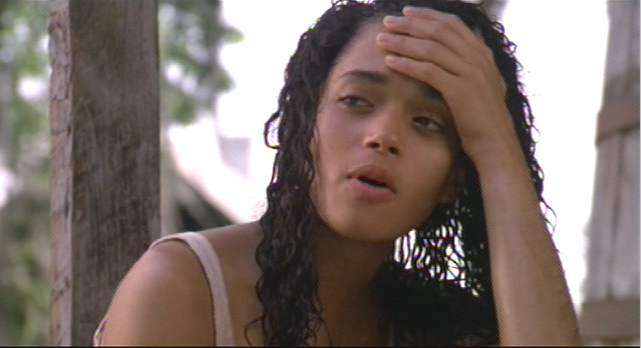
\includegraphics[width=\textwidth]{images/datasets/frame.25.png}
         \caption{}
         \label{fig:lvs-gt-x}
     \end{subfigure}
     \hfill
     \begin{subfigure}[b]{0.3\textwidth}
         \centering
         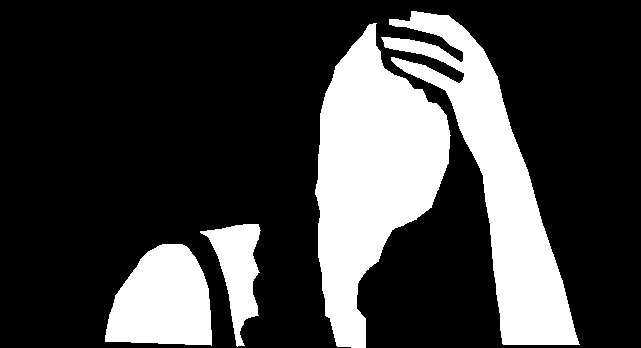
\includegraphics[width=\textwidth]{images/datasets/skin.25.png}
         \caption{}
         \label{fig:lvs-gt-skin}
     \end{subfigure}
    \hfill
     \begin{subfigure}[b]{0.3\textwidth}
         \centering
         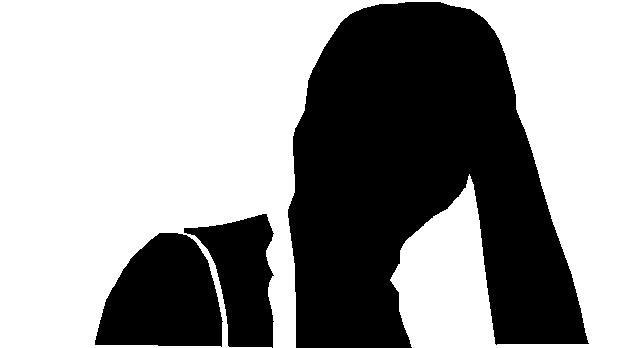
\includegraphics[width=\textwidth]{images/datasets/background.25.png}
         \caption{}
         \label{fig:lvs-gt-noskin}
     \end{subfigure}
        \caption{LVS~\cite{jones2002statistical} dataset example: (a) original image, (b) skin ground truth, (c) non-skin ground truth.
        Facial features like the eyes and mouth are treated as skin.}
        \label{fig:lvs-gt}
\end{figure}


%%%%%%%%%%%%%%%%%%%%%%%%%%%%%%%%%%%%%%%%%%%%%%%%%%%%%%%%%%%%%%%%%%%%%%%%
\section{Issues}
%%%%%%%%%%%%%%%%%%%%%%%%%%%%%%%%%%%%%%%%%%%%%%%%%%%%%%%%%%%%%%%%%%%%%%%%

Image databases are essential for developing skin detectors.
Over the years, new databases keep getting published, but there are still some limitations on their reliability.\\
The major limitations are described below, and some of them are illustrated in \autoref{fig:tdsd-gt}.

\begin{itemize}
    \item The number of pictures is sometimes not sufficiently high.
    \item The image quality is at times very low, and a sufficient intra-class variation is not present.
    \item The classes are often unbalanced, with one being much larger than the other, which may cause some metrics to give overoptimistic estimations~\cite{chicco2020advantages}.
    \item The ground truth labeling sometimes is performed using semi-automatic techniques, which give imprecise results~\cite{mahmoodi2015sdd}.
    Moreover, some skin regions are of dubious classification, especially the boundaries of the skin and around features such as eyes and mouth.
    \item Additional data is often cited in the original papers of the datasets, but not provided alongside it. Data about the lighting conditions, background complexity, number of subjects, indoor or outdoor scenery of an image may be extremely useful in some applications.
    \item Compression artifacts generated during the storage of ground truth masks represent another issue. The artifacts are inconvenient for either binary and segmentation masks and should be avoided by using lossless formats.
    \item Different skin tones are rarely evenly represented, and especially are not directly labeled.
    Furthermore, the categorization of skin tones does not follow a standard system and is questionable.
    \item Most image databases do not provide native training and testing splits, which confuses the evaluations in the literature.
\end{itemize}

\begin{figure}[!hbt]
     \centering
     \begin{subfigure}[b]{0.25\textwidth}
         \centering
         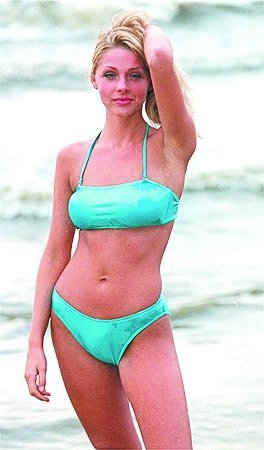
\includegraphics[width=\textwidth]{images/datasets/0487.jpg}
         \caption{}
         \label{fig:tdsd-gt-x}
     \end{subfigure}
     \hfill
     \begin{subfigure}[b]{0.25\textwidth}
         \centering
         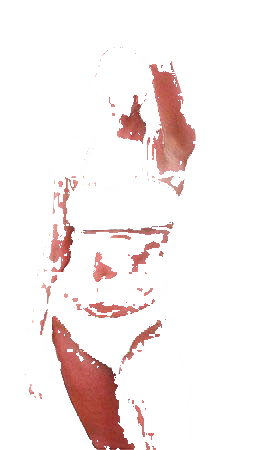
\includegraphics[width=\textwidth]{images/datasets/0487.png}
         \caption{}
         \label{fig:tdsd-gt-skin}
     \end{subfigure}
     \hfill
     \begin{subfigure}[b]{0.4\textwidth}
         \centering
         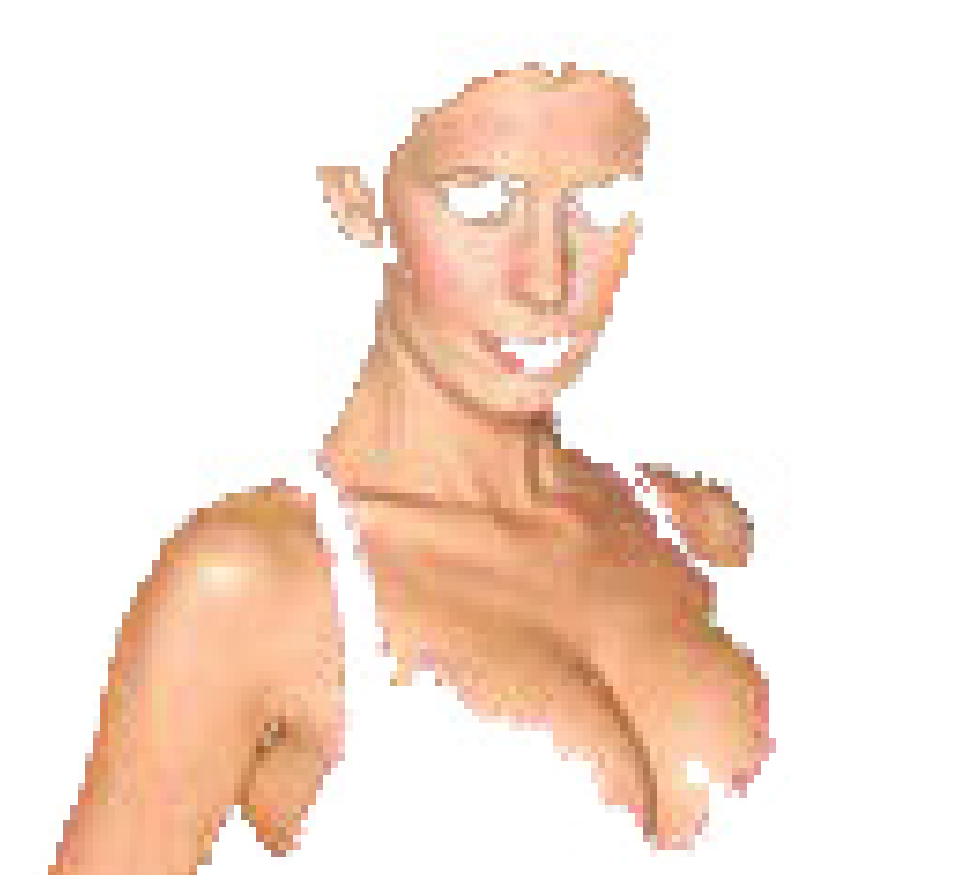
\includegraphics[width=\textwidth]{images/datasets/tdsd_artifacts.png}
         \caption{}
         \label{fig:tdsd-gt-noskin}
     \end{subfigure}
        \caption{TDSD~\cite{zhu2004adaptive} bad annotation examples: (a) original image No. 0487; (b) skin segmentation ground truth No. 0487; (c) compression artifacts.
        Test Database for Skin Detection (TDSD) contains both good and bad annotation examples. Ruiz-del-Solar and Verschae proposed three sub-dataset splits based on the annotation quality~\cite{ruiz2006skindiff}.
        Despite the issues, the dataset is important because, being born as a test dataset, it contains more uncorrelated images than those available in video datasets~\cite{bianco2015adaptive}.}
        \label{fig:tdsd-gt}
\end{figure}

%%%%%%%%%%%%%%%%%%%%%%%%%%%%%%%%%%%%%%%%%%%%%%%%%%%%%%%%%%%%%%%%%%%%%%%%
\section{Chosen Datasets}\label{sec:chosen-datasets}
%%%%%%%%%%%%%%%%%%%%%%%%%%%%%%%%%%%%%%%%%%%%%%%%%%%%%%%%%%%%%%%%%%%%%%%%

Accordingly to the issues previously mentioned, and considering the popularity, diversity, and size of the databases, the selected datasets for this work are ECU~\cite{phung2005skin}, HGR~\cite{Kawulok2014EURASIP} and Schmugge~\cite{schmugge2007objective}. A more detailed description of each one follows.

\noindent\textbf{ECU}~\cite{phung2005skin} is a dataset created at the Edith Cowan University that aims to support research on skin segmentation and face detection.
It contains 3998 pictures differing in terms of the depicted skin regions, skin tone types, lighting, and background, with both indoor and outdoor environments.
The authors did a rough categorization of the skin tones: 1665 images represent whitish and pinkish skin types; 1402 images represent yellowish and light brownish skin types; 965 images characterize reddish, darkish, and dark brownish skin types; the remaining ones generically represent other skin types.\\
\textbf{HGR}~\cite{Kawulok2014EURASIP} is a Hand Gesture Recognition Database of 1558 images. It organizes into three different sub-datasets: HGR1, HGR2A, and HGR2B.
HGR1 is a set of 899 pictures of various sizes and taken in uncontrolled light and background environments.
HGR2A contains 85 images of the same dimension taken in uniform lighting and both controlled and uncontrolled backgrounds.
HGR2B features 574 constant-sized pictures taken with a controlled background and in uniform lighting.
The skin tone diversity is very low as the images represent only a limited number of subjects.
Regarding the HGR2A and HGR2B sub-datasets, this work utilizes the downscaled versions of the pictures because high-resolution images would automatically be downscaled in approaches like neural networks.\\
\textbf{Schmugge}~\cite{schmugge2007objective} takes the name from its creator and consists of 845 images taken from different sources: the pictures representing skin pixels are collected from the AR face dataset~\cite{martinez1998ar}, the UOPB dataset~\cite{marszalec2000physics}, and the University of Chile dataset~\cite{ruiz2006skindiff}.
The first two include frontal facial images with varying illumination conditions and a very plain white background. Therefore, for these images, the non-skin pixels are not included.
The Chile dataset is composed of websites and digitized news clips and represents a variety of scenes, thus its non-skin pixels are included.
Other non-skin pixels are collected by randomly sampling the University of Washington content-based image retrieval database~\cite{berman1999flexible}.
Unlike other datasets, the ground truth follows a ternary representation: pixels are labeled as skin, non-skin, and \q{don't care}.
The \q{don’t care} label is assigned to pixels that are too ambiguous or tedious to label as either skin or non-skin.
This ternary division permits better management of pixels classification.
The dataset provides different files featuring additional data for each image, such as the skin tone, the light type, and the original database the picture is from. The ternary annotation system used in the dataset is shown in \autoref{fig:schmugge-ternary}.

\begin{figure}[hb]
    \centering
    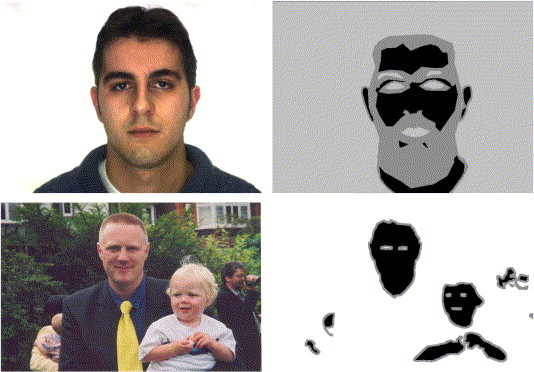
\includegraphics[width=0.7\linewidth]{images/datasets/schmugge_sample.jpg}
    \caption{Schmugge~\cite{schmugge2007objective} samples, RGB image on the left column and groundtruth on the right column. In annotations, skin pixels are black while non-skin pixels are white.
    Difficult and tedious regions to mark (\q{don’t care}) are colored in gray.
    The background in the top two images is marked in gray, indicating that those pixels did not participate in the evaluation. Adapted from Schmugge \textit{et al.} 2007~\cite{schmugge2007objective}}
    \label{fig:schmugge-ternary}
\end{figure}
